\documentclass[aspectratio=169,11pt]{beamer}
\usetheme{Madrid}
\usecolortheme{default}
\setbeamertemplate{navigation symbols}{}
\usepackage{booktabs}
\usepackage{pgfplots}
\pgfplotsset{compat=1.17}
\usetikzlibrary{positioning,arrows.meta}

\title[Advisory vs.\ Enforced Agreement]{Where Dialog-Only Coordination Breaks:\\Advisory vs.\ Enforced Agreement for LLM Agents}
\subtitle{Weekly Research Report}
\author{Chiharu Tomimori}
\institute{Institute of Science Tokyo}
\date{November 6, 2026}

\newcommand{\papercite}[1]{%
  \vfill
  \begin{beamercolorbox}[wd=\textwidth,sep=3pt]{block body}
    \tiny #1
  \end{beamercolorbox}}
\tikzset{
  box/.style={draw, rounded corners, fill=blue!8, minimum height=1.0cm, text width=2.3cm, align=center, font=\footnotesize},
  hl/.style={box, fill=orange!20},
  arr/.style={-{Stealth[length=2mm]}, thick}
}
% colors used in every chart, always in the order baseline, advisory, enforced
\definecolor{cbase}{RGB}{150,150,150}
\definecolor{cadv}{RGB}{70,120,200}
\definecolor{cenf}{RGB}{220,120,40}

\begin{document}

% ===============================================================
\begin{frame}
  \titlepage
\end{frame}

% ===============================================================
\section{Last Week}
\begin{frame}{Last Week (Oct 30): Feedback and What I Did}
  \small
  \begin{tabular}{p{6.6cm}p{6.6cm}}
    \toprule
    Feedback & What I did this week \\
    \midrule
    Accuracy or time? & accuracy is the main metric; time is secondary \\
    \leavevmode\pause Need a baseline & same tool for all; baseline has no rule \\
    \leavevmode\pause Context loss and crash are reversed & fixed: crash loses \textbf{new}, context loss loses \textbf{old} \\
    \leavevmode\pause ``Skill'' and ``harness'' are unclear & new terms: \textbf{advisory} and \textbf{enforced} \\
    \leavevmode\pause Three-way comparison (none / naive / proposed) & postponed; first find where dialog breaks \\
    \leavevmode\pause Presentation (one message per slide, order, et al.) & applied to all slides \\
    \bottomrule
  \end{tabular}

  \vspace{0.5em}
  \pause\footnotesize Every number in this talk is a \textbf{success} count unless marked.
\end{frame}

% ---------------------------------------------------------------

% ===============================================================
\section{Progress}
\begin{frame}{Progress in This Week: Overview}
  \centering
  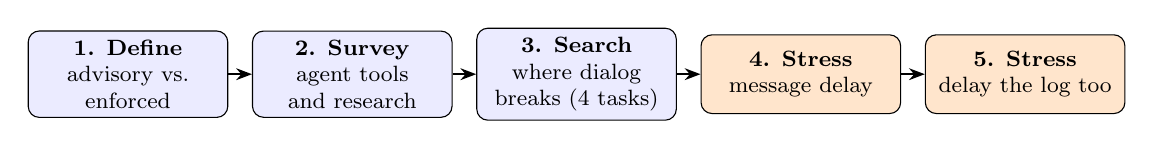
\begin{tikzpicture}[node distance=0.3cm]
    \node[box] (a) {\textbf{1. Define}\\advisory vs.\ enforced};
    \node[box, right=of a] (b) {\textbf{2. Survey}\\agent tools and research};
    \node[box, right=of b] (c) {\textbf{3. Search}\\where dialog breaks (4 tasks)};
    \node[hl, right=of c] (d) {\textbf{4. Stress}\\message delay};
    \node[hl, right=of d] (e) {\textbf{5. Stress}\\delay the log too};
    \draw[arr] (a)--(b); \draw[arr] (b)--(c); \draw[arr] (c)--(d); \draw[arr] (d)--(e);
  \end{tikzpicture}

  \vspace{1em}
  \pause
  \small
  \textbf{Main findings}
  \begin{itemize}
    \item With slow, asynchronous communication, dialog alone fails; the agreement procedure still succeeds
    \pause
    \item Advisory and enforced differ in \textbf{how} they fail, not in how often
  \end{itemize}
\end{frame}

% ===============================================================
\subsection{Introduction}
\begin{frame}{Background and Motivation}
  \small
  \begin{itemize}
    \item First 4 tasks this week: baseline succeeded in \textbf{20 / 20} runs\\
      $\Rightarrow$ dialog was enough; no gap to close (ceiling effect)
    \pause
    \item \textbf{Question}: when does dialog alone break, and does an agreement procedure prevent it?
    \pause
    \item \textbf{Focus}: not only agreeing, but \textbf{acting by the agreement afterwards} (conformance)
  \end{itemize}
\end{frame}

% ---------------------------------------------------------------
\begin{frame}{Related Work: How Existing Agent Tools Coordinate}
  \scriptsize
  \begin{tabular}{p{3.3cm}p{6.3cm}p{4.0cm}}
    \toprule
    Tool & How agents coordinate & Commit a shared choice? \\
    \midrule
    LangGraph [1] & shared state; reducers merge concurrent updates & no (merge) \\
    \leavevmode\pause AutoGen [2] & conversation; a manager picks the next speaker & no (dialog only) \\
    \leavevmode\pause CrewAI [3] & a manager agent delegates & no (manager decides) \\
    \leavevmode\pause OpenAI Agents SDK [4] & handoffs: one agent in control at a time & no (no parallel owners) \\
    \leavevmode\pause A2A protocol [5] & messages and tasks between agents & no (transport only) \\
    \leavevmode\pause Claude Code teams [6] & fixed lead; task list with file lock; mailbox & no (lock for tasks only) \\
    \bottomrule
  \end{tabular}

  \vspace{0.2em}
  \pause
  Research: BFT votes on answers [7, 8]; transactions for plans [9]; failures measured, no talk [10]\\
  \textbf{This work}: commit a shared choice, then check that each agent follows it.
  \papercite{
  [1] LangChain, LangGraph documentation, https://docs.langchain.com/oss/python/langgraph/overview (accessed Nov.\ 2026).\\
  {}[2] Q.\ Wu et al., ``AutoGen: Enabling Next-Gen LLM Applications via Multi-Agent Conversation,'' in \textit{Proc.\ COLM}, 2024.\\
  {}[3] CrewAI, CrewAI documentation: Processes, https://docs.crewai.com (accessed Nov.\ 2026).\\
  {}[4] OpenAI, OpenAI Agents SDK documentation: Handoffs, https://openai.github.io/openai-agents-python/handoffs/ (accessed Nov.\ 2026).\\
  {}[5] Agent2Agent (A2A) Protocol specification, https://a2a-protocol.org (accessed Nov.\ 2026).\\
  {}[6] Anthropic, ``Orchestrate teams of Claude Code sessions,'' https://code.claude.com/docs/en/agent-teams (accessed Nov.\ 2026).\\
  {}[7] L.\ Zheng et al., ``Rethinking the Reliability of Multi-agent System: A Perspective from Byzantine Fault Tolerance,'' arXiv:2511.10400 (preprint), 2025.\\
  {}[8] Y.\ Jo et al., ``Byzantine-Robust Decentralized Coordination of LLM Agents,'' arXiv:2507.14928 (preprint), 2025.\\
  {}[9] E.\ Y.\ Chang et al., ``SagaLLM: Context Management, Validation, and Transaction Guarantees for Multi-Agent LLM Planning,'' \textit{PVLDB}, vol.\ 18, no.\ 12, 2025.\\
  {}[10] C.\ Chac\'on Sartori, ``The Specification Gap: Coordination Failure Under Partial Knowledge in Code Agents,'' arXiv:2603.24284 (preprint), 2026.}
\end{frame}

% ===============================================================
\subsection{Methods}
\begin{frame}{Model: Agents, Channels, Timing}
  \small
  \begin{tabular}{p{3.0cm}p{10.2cm}}
    \toprule
    Part & Assumption \\
    \midrule
    Agents & 3 LLM agents; each owns one module; no shared files \\
    \leavevmode\pause Channels & message board (broadcast) + shared decision log \\
    \leavevmode\pause Failures & no crash; an agent may \textbf{finish and leave early} \\
    \leavevmode\pause Timing & each message is delayed 0--150\,s; agents do \textbf{not} know the delay \\
    \leavevmode\pause Base method & atomic commit [12]: a decision is final only when \textbf{all} participants accept \\
    \leavevmode\pause Tool & \texttt{propose}, \texttt{respond}, \texttt{commit}, \texttt{lookup}, \texttt{withdraw}, \texttt{leave}; append-only log \\
    \bottomrule
  \end{tabular}

  \vspace{0.6em}
  \pause\small
  Timing = partial synchrony [11] (bounded delay, bound unknown).
  \papercite{
  [11] C.\ Dwork et al., ``Consensus in the Presence of Partial Synchrony,'' \textit{Journal of the ACM}, vol.\ 35, no.\ 2, pp.\ 288--323, 1988.\\
  {}[12] J.\ Gray, ``Notes on Data Base Operating Systems,'' in \textit{Operating Systems: An Advanced Course}, LNCS vol.\ 60, pp.\ 393--481, Springer, 1978.}
\end{frame}

% ---------------------------------------------------------------
\begin{frame}{Proposed Method (Overview): Advisory vs.\ Enforced}
  \small
  \textbf{Rule}: ``Do not write your file until $\geq$1 decision is committed and none is open.
  Then follow the decisions, even against your own habits.''
  \vspace{0.5em}

  \begin{tabular}{p{3.6cm}p{3.0cm}p{3.0cm}p{3.0cm}}
    \toprule
    & Baseline & Advisory & Enforced \\
    \midrule
    Agreement tool & yes & yes & yes \\
    \leavevmode\pause Rule in the prompt & no & \textbf{yes} & no \\
    \leavevmode\pause Hook blocks early writes & no & no & \textbf{yes} \\
    \leavevmode\pause Who applies the rule & --- & the model & the runtime \\
    \bottomrule
  \end{tabular}

  \vspace{0.5em}
  \pause\footnotesize Enforced shows the rule text only when a write is blocked.
\end{frame}

% ---------------------------------------------------------------

% ---------------------------------------------------------------
\begin{frame}{Task: Three Modules, Three Conflicting Standards}
  \small
  Build an invoice: \texttt{pricing.py} (agent 1), \texttt{tax.py} (agent 2), \texttt{invoice.py} (agent 3)
  \vspace{0.4em}

  \begin{tabular}{p{2.6cm}p{3.4cm}p{3.4cm}p{3.6cm}}
    \toprule
    Standard & Agent 1 & Agent 2 & Agent 3 \\
    \midrule
    Money & float dollars & int cents & Decimal dollars \\
    Percent & fraction (0.10) & number (10) & multiplier (0.90) \\
    Not found & \texttt{None} & \texttt{KeyError} & default value \\
    \bottomrule
  \end{tabular}

  \vspace{0.6em}
  \pause
  \begin{itemize}
    \item APIs between modules are \textbf{not given}: the agents decide them
    \pause
    \item Success = all \textbf{14 hidden tests} pass after the three files are merged
    \pause
    \item Similar designs: information split across agents [13, 14]; conflicting parallel parts [15]
  \end{itemize}
  \papercite{
  [13] G.\ Stasser et al., ``Pooling of Unshared Information in Group Decision Making,'' \textit{Journal of Personality and Social Psychology}, vol.\ 48, no.\ 6, pp.\ 1467--1478, 1985.\\
  {}[14] Y.\ Li et al., ``Systematic Failures in Collective Reasoning under Distributed Information in Multi-Agent LLMs,'' in \textit{Proc.\ ICML}, PMLR 306, 2026.\\
  {}[15] A.\ Khatua et al., ``CooperBench: Why Coding Agents Cannot be Your Teammates Yet,'' arXiv:2601.13295 (preprint), 2026.}
\end{frame}

% ---------------------------------------------------------------
\begin{frame}{Stress Conditions: Making Communication Slow}
  \small
  \begin{tabular}{p{3.4cm}p{3.4cm}p{3.4cm}p{2.6cm}}
    \toprule
    Stress & Message board & Decision log & Runs per cond. \\
    \midrule
    None & no delay & no delay & 5 \\
    \leavevmode\pause Short delay & 20--60\,s & no delay & 10 / 5 / 5 \\
    \leavevmode\pause Long delay & 60--150\,s & no delay & 10 \\
    \leavevmode\pause Long delay, both & 60--150\,s & 60--150\,s & 10 \\
    \bottomrule
  \end{tabular}

  \vspace{0.6em}
  \pause\footnotesize
  Delay is random per entry; the writer sees its own entry at once. Delayed log: correct but slow.

  \vspace{0.4em}
  \textbf{Environment}
  \begin{itemize}\setlength{\itemsep}{0pt}
    \item Agent runtime: Claude Code 2.1.318, non-interactive mode (\texttt{claude -p})
    \item Model: Claude Haiku for all agents
    \item Limits: 60 turns per agent, 30 min per run
    \item Machine: cloud container, 2 vCPU (Xeon 2.1\,GHz), 7\,GB RAM, no GPU
    \item Software: Python 3.13
  \end{itemize}
\end{frame}

% ---------------------------------------------------------------

% ===============================================================
\subsection{Results}

% ---------------------------------------------------------------
\begin{frame}{Result 1: Success Rate Under Delay}
  \centering
  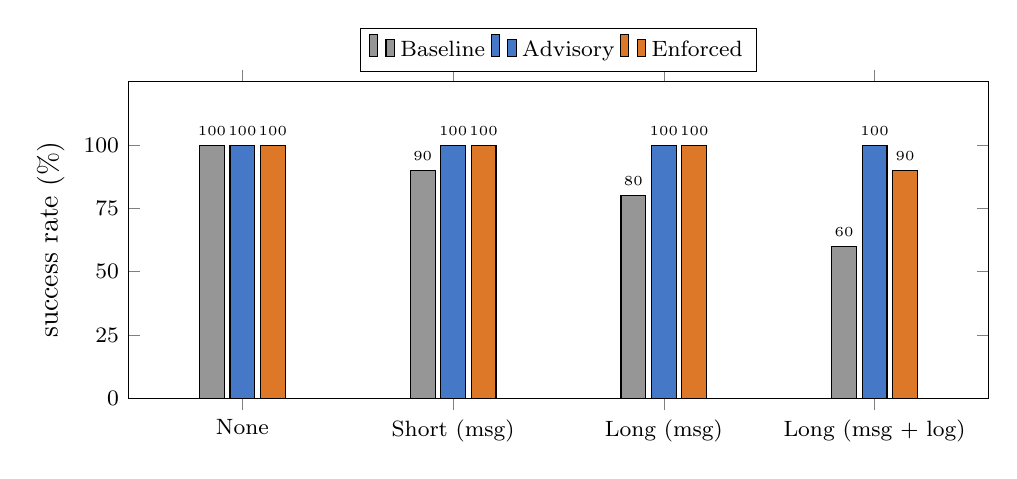
\begin{tikzpicture}
    \begin{axis}[
      ybar, bar width=9pt, width=12.5cm, height=5.6cm,
      ymin=0, ymax=125, ytick={0,25,50,75,100}, ylabel={success rate (\%)},
      symbolic x coords={None,Short,Long,Long both},
      xtick=data, xticklabels={None, {Short (msg)}, {Long (msg)}, {Long (msg + log)}},
      nodes near coords, nodes near coords style={font=\tiny},
      legend style={at={(0.5,1.03)}, anchor=south, legend columns=3, font=\footnotesize},
      enlarge x limits=0.18, tick label style={font=\footnotesize}]
      \addplot[fill=cbase] coordinates {(None,100) (Short,90) (Long,80) (Long both,60)};
      \addplot[fill=cadv]  coordinates {(None,100) (Short,100) (Long,100) (Long both,100)};
      \addplot[fill=cenf]  coordinates {(None,100) (Short,100) (Long,100) (Long both,90)};
      \legend{Baseline, Advisory, Enforced}
    \end{axis}
  \end{tikzpicture}

  \footnotesize Long, both (10 runs each): baseline 6, advisory 10, enforced 9 successes.
\end{frame}

% ---------------------------------------------------------------
\begin{frame}{Result 2: Why the Baseline Failed}
  \small
  \textbf{The 6 baseline failures under long delay share one pattern}
  \vspace{0.4em}

  \begin{tabular}{p{1.4cm}p{9.6cm}p{2.0cm}}
    \toprule
    Step & What happened & Runs \\
    \midrule
    1 & agent 1 or 2 sends its API and stops within 50\,s & 6 / 6 \\
    \leavevmode\pause 2 & agent 3 writes \texttt{invoice.py} \textbf{before} those messages arrive & 5 / 6 \\
    \leavevmode\pause 3 & agent 3 \textbf{guesses} function names & --- \\
    \leavevmode\pause 4 & merge fails: e.g.\ \texttt{pricing} has no attribute \texttt{customer\_name} & 6 / 6 \\
    \bottomrule
  \end{tabular}

  \vspace{0.6em}
  \pause
  Commit works as a \textbf{barrier}: nobody writes until everyone has accepted.
\end{frame}

% ---------------------------------------------------------------

% ---------------------------------------------------------------
\begin{frame}{Result 3: Advisory and Enforced Fail Differently}
  \small
  \begin{tabular}{p{3.2cm}p{4.8cm}p{4.8cm}}
    \toprule
    & Baseline failure (4 runs) & Enforced failure (1 run) \\
    \midrule
    What happened & wrote parts that do not fit & wrote nothing; stopped \\
    \leavevmode\pause Property broken & \textbf{safety} (wrong result) & \textbf{liveness} (no result) \\
    \leavevmode\pause Cause & guessed API under delay & proposals replaced again and again \\
    \bottomrule
  \end{tabular}

  \vspace{0.6em}
  \pause\footnotesize
  Enforced run 9: 17 proposals, 14 aborted or withdrawn, 0 commits (float dollars $\leftrightarrow$ int cents).\\
  New versions arrived before votes on old ones were visible $\Rightarrow$ livelock, like duelling proposers in Paxos [16].
  \papercite{[16] L.\ Lamport, ``The Part-Time Parliament,'' \textit{ACM Transactions on Computer Systems}, vol.\ 16, no.\ 2, pp.\ 133--169, 1998.}
\end{frame}

% ---------------------------------------------------------------

% ===============================================================
\subsection{Discussion}
\begin{frame}{Discussion: What This Week Shows}
  \small
  \begin{itemize}
    \item Earlier tasks: the baseline never failed $\Rightarrow$ the problem was the \textbf{task}, not the method
    \pause
    \item This week: built a task where the baseline \textbf{does} fail (100\,\% $\to$ 60\,\% success under slow communication)
    \pause
    \item The procedure prevents it even with a slow log: the benefit is the \textbf{barrier}, not a fast log
    \pause
    \item Cost is time: about $2.5\times$ the baseline with a slow log (696 / 735\,s vs.\ 272\,s)
    \pause
    \item Advisory agents mostly obeyed the rule: 0 / 10 runs wrote before any commit
  \end{itemize}
\end{frame}

% ---------------------------------------------------------------
\begin{frame}{Next Week}
  \small
  \begin{enumerate}
    \item \textbf{Remove the confound}: enforced = advisory rule in prompt + hook
    \pause
    \item \textbf{Make rule-breaking costly}: a late objection arrives just before commit
    \begin{itemize}
      \item an agent that writes too early must fail
      \item expected: advisory sometimes fails, enforced blocks it
    \end{itemize}
    \pause
    \item Count would-be violations for both conditions with the same metric
  \end{enumerate}
\end{frame}

% ===============================================================
\section{Questions}
\begin{frame}{Question List}
  \small
  \begin{enumerate}
    \item Is ``bounded but unknown message delay'' a convincing model of asynchronous LLM agents?
    \pause
    \item Should liveness failures (no output) count the same as wrong output?
    \pause
    \item Is it fair that enforced hides the rule until a block, or should both conditions see it?
    \pause
    \item Is 10 runs per condition enough for a first paper, or should I aim for 20--30?
  \end{enumerate}
\end{frame}

\end{document}
